\chapter{Evaluation and experiments}
\section{Single Quadrotor Control with Payload}
\begin{itemize}
    \item Recover from harsh and track position
    \item Follow trajectory
    \item Follow trajectory with disturbance
    \item Sim2Real
    \item Plots: Recovery success rate for 10000 rollouts ofver time.
    \item Plots: Trajectory following 3d, error over time for batch

\end{itemize}
\begin{figure}
    \centering
    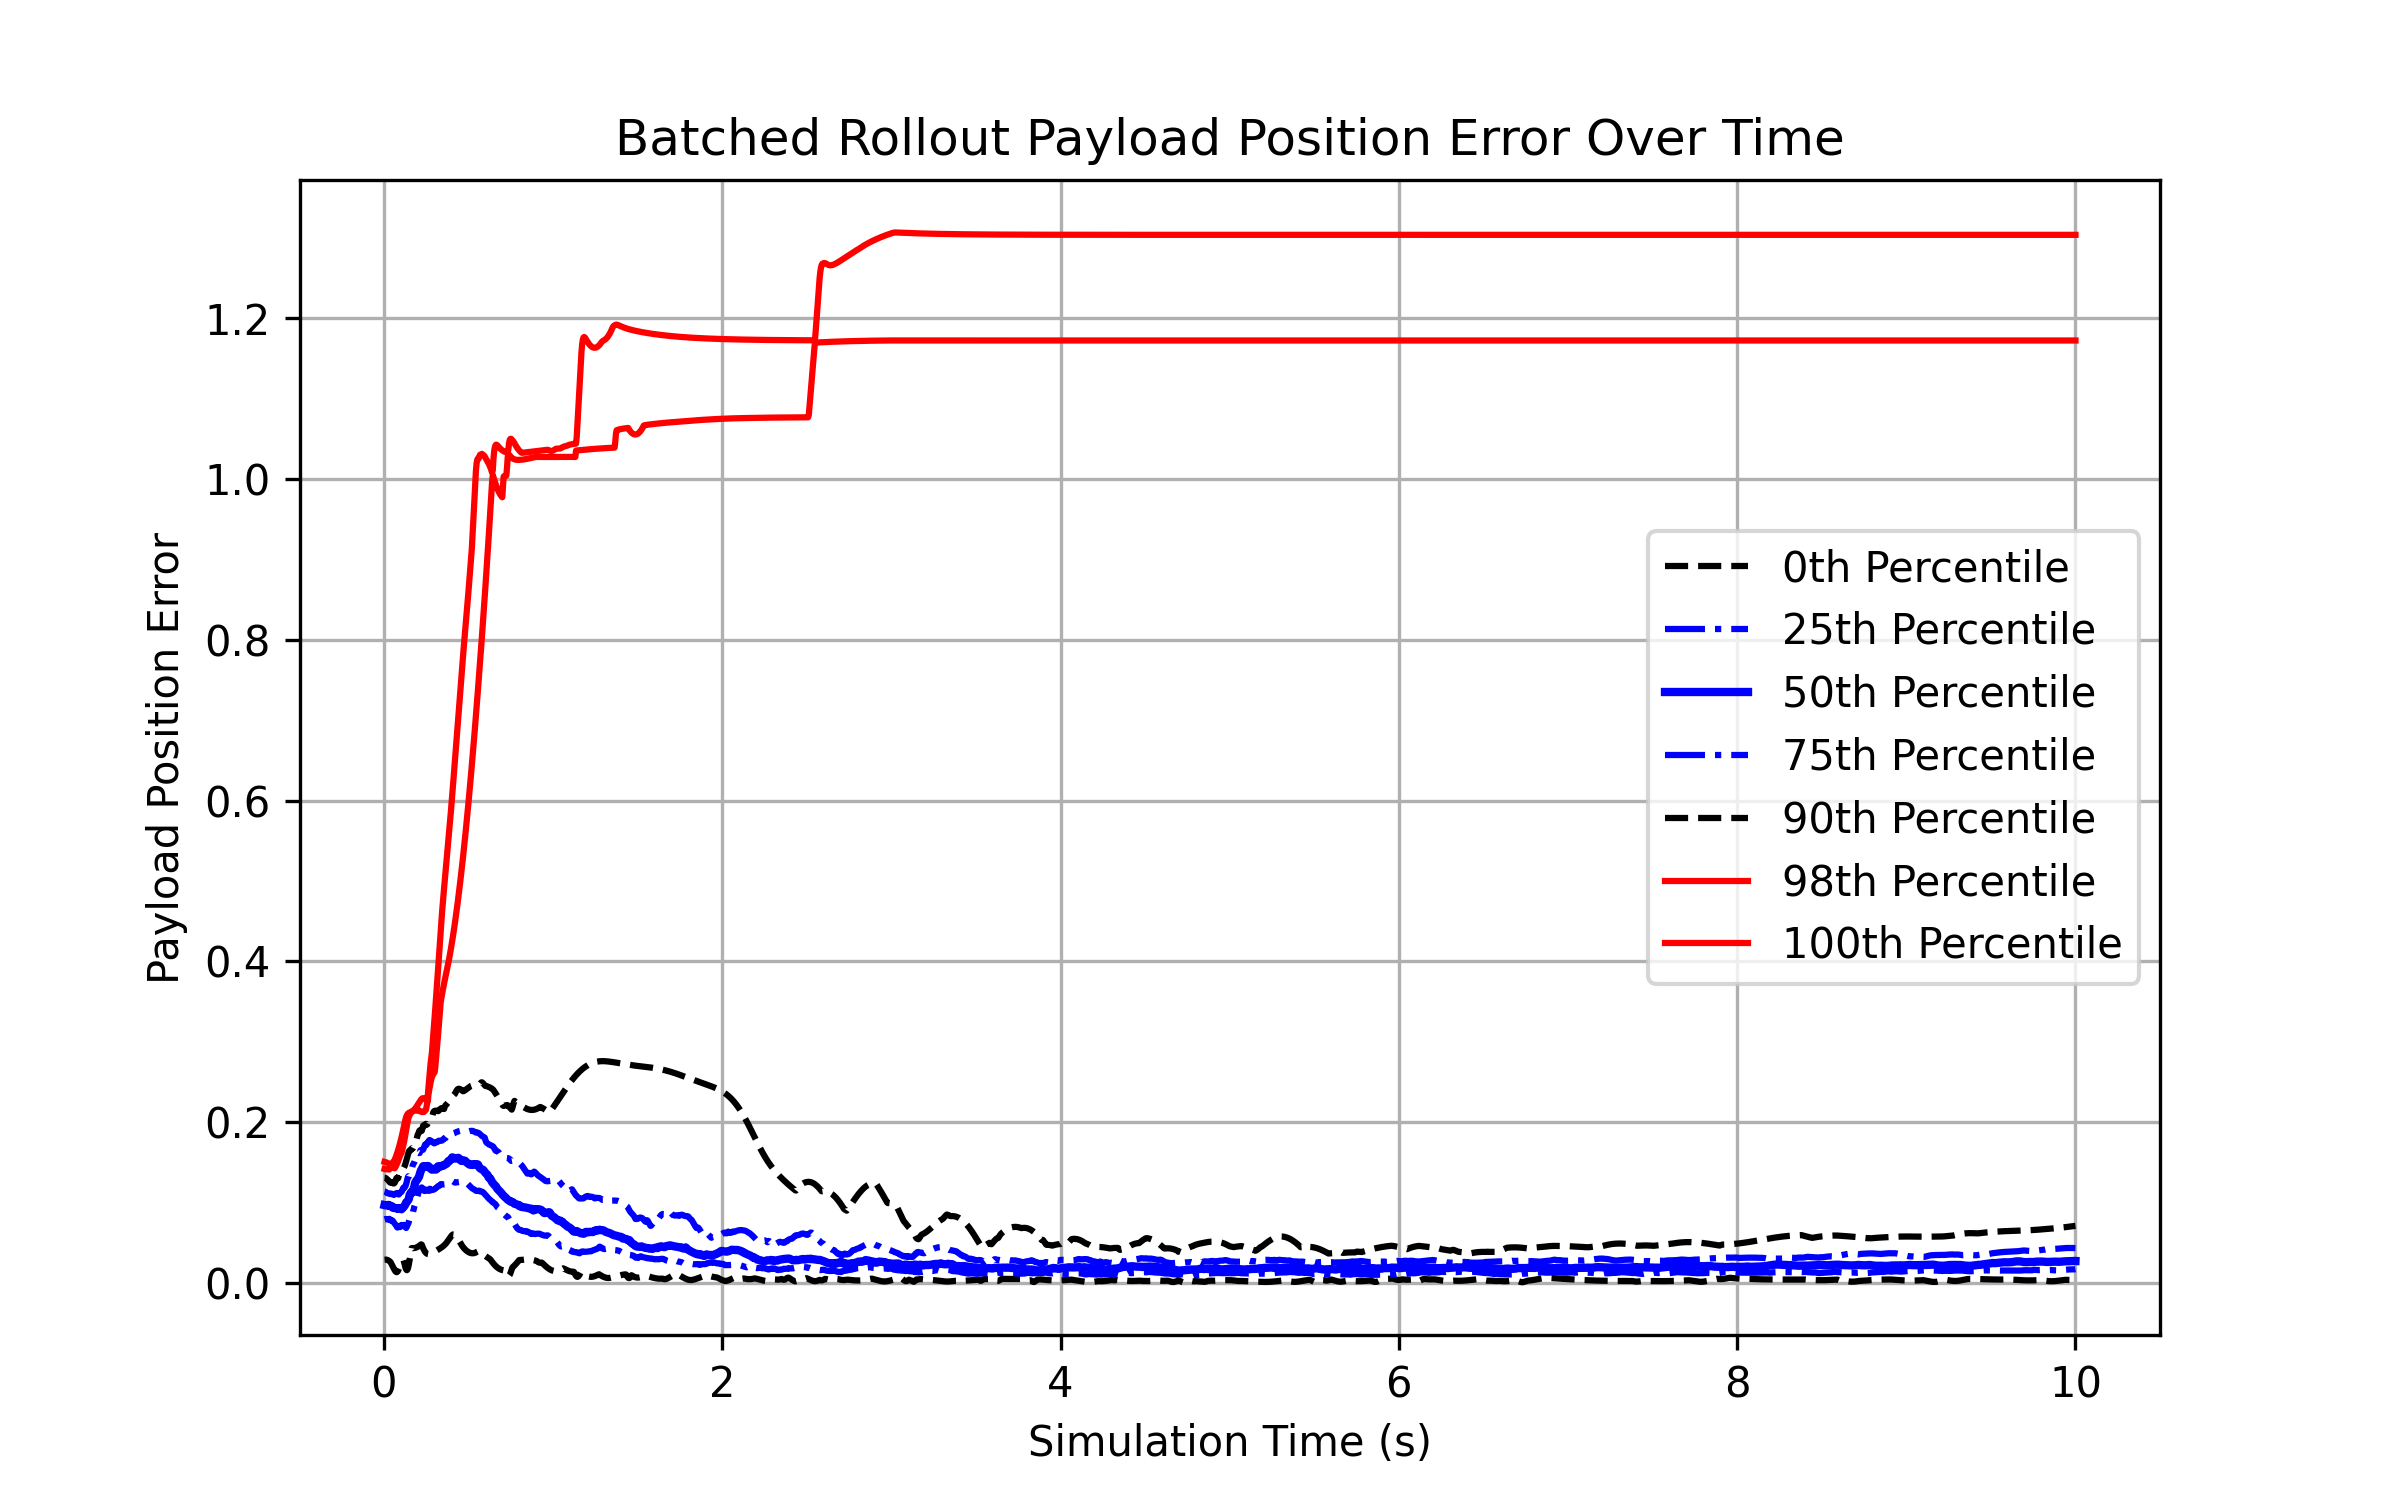
\includegraphics[width=\textwidth]{batch.png}
    \caption{Single quadrotor control with payload. The quadrotor is able to recover from harsh disturbances and track a desired position.}
    \label{fig:single_quadrotor_control}
\end{figure}
\begin{figure}
    \centering
    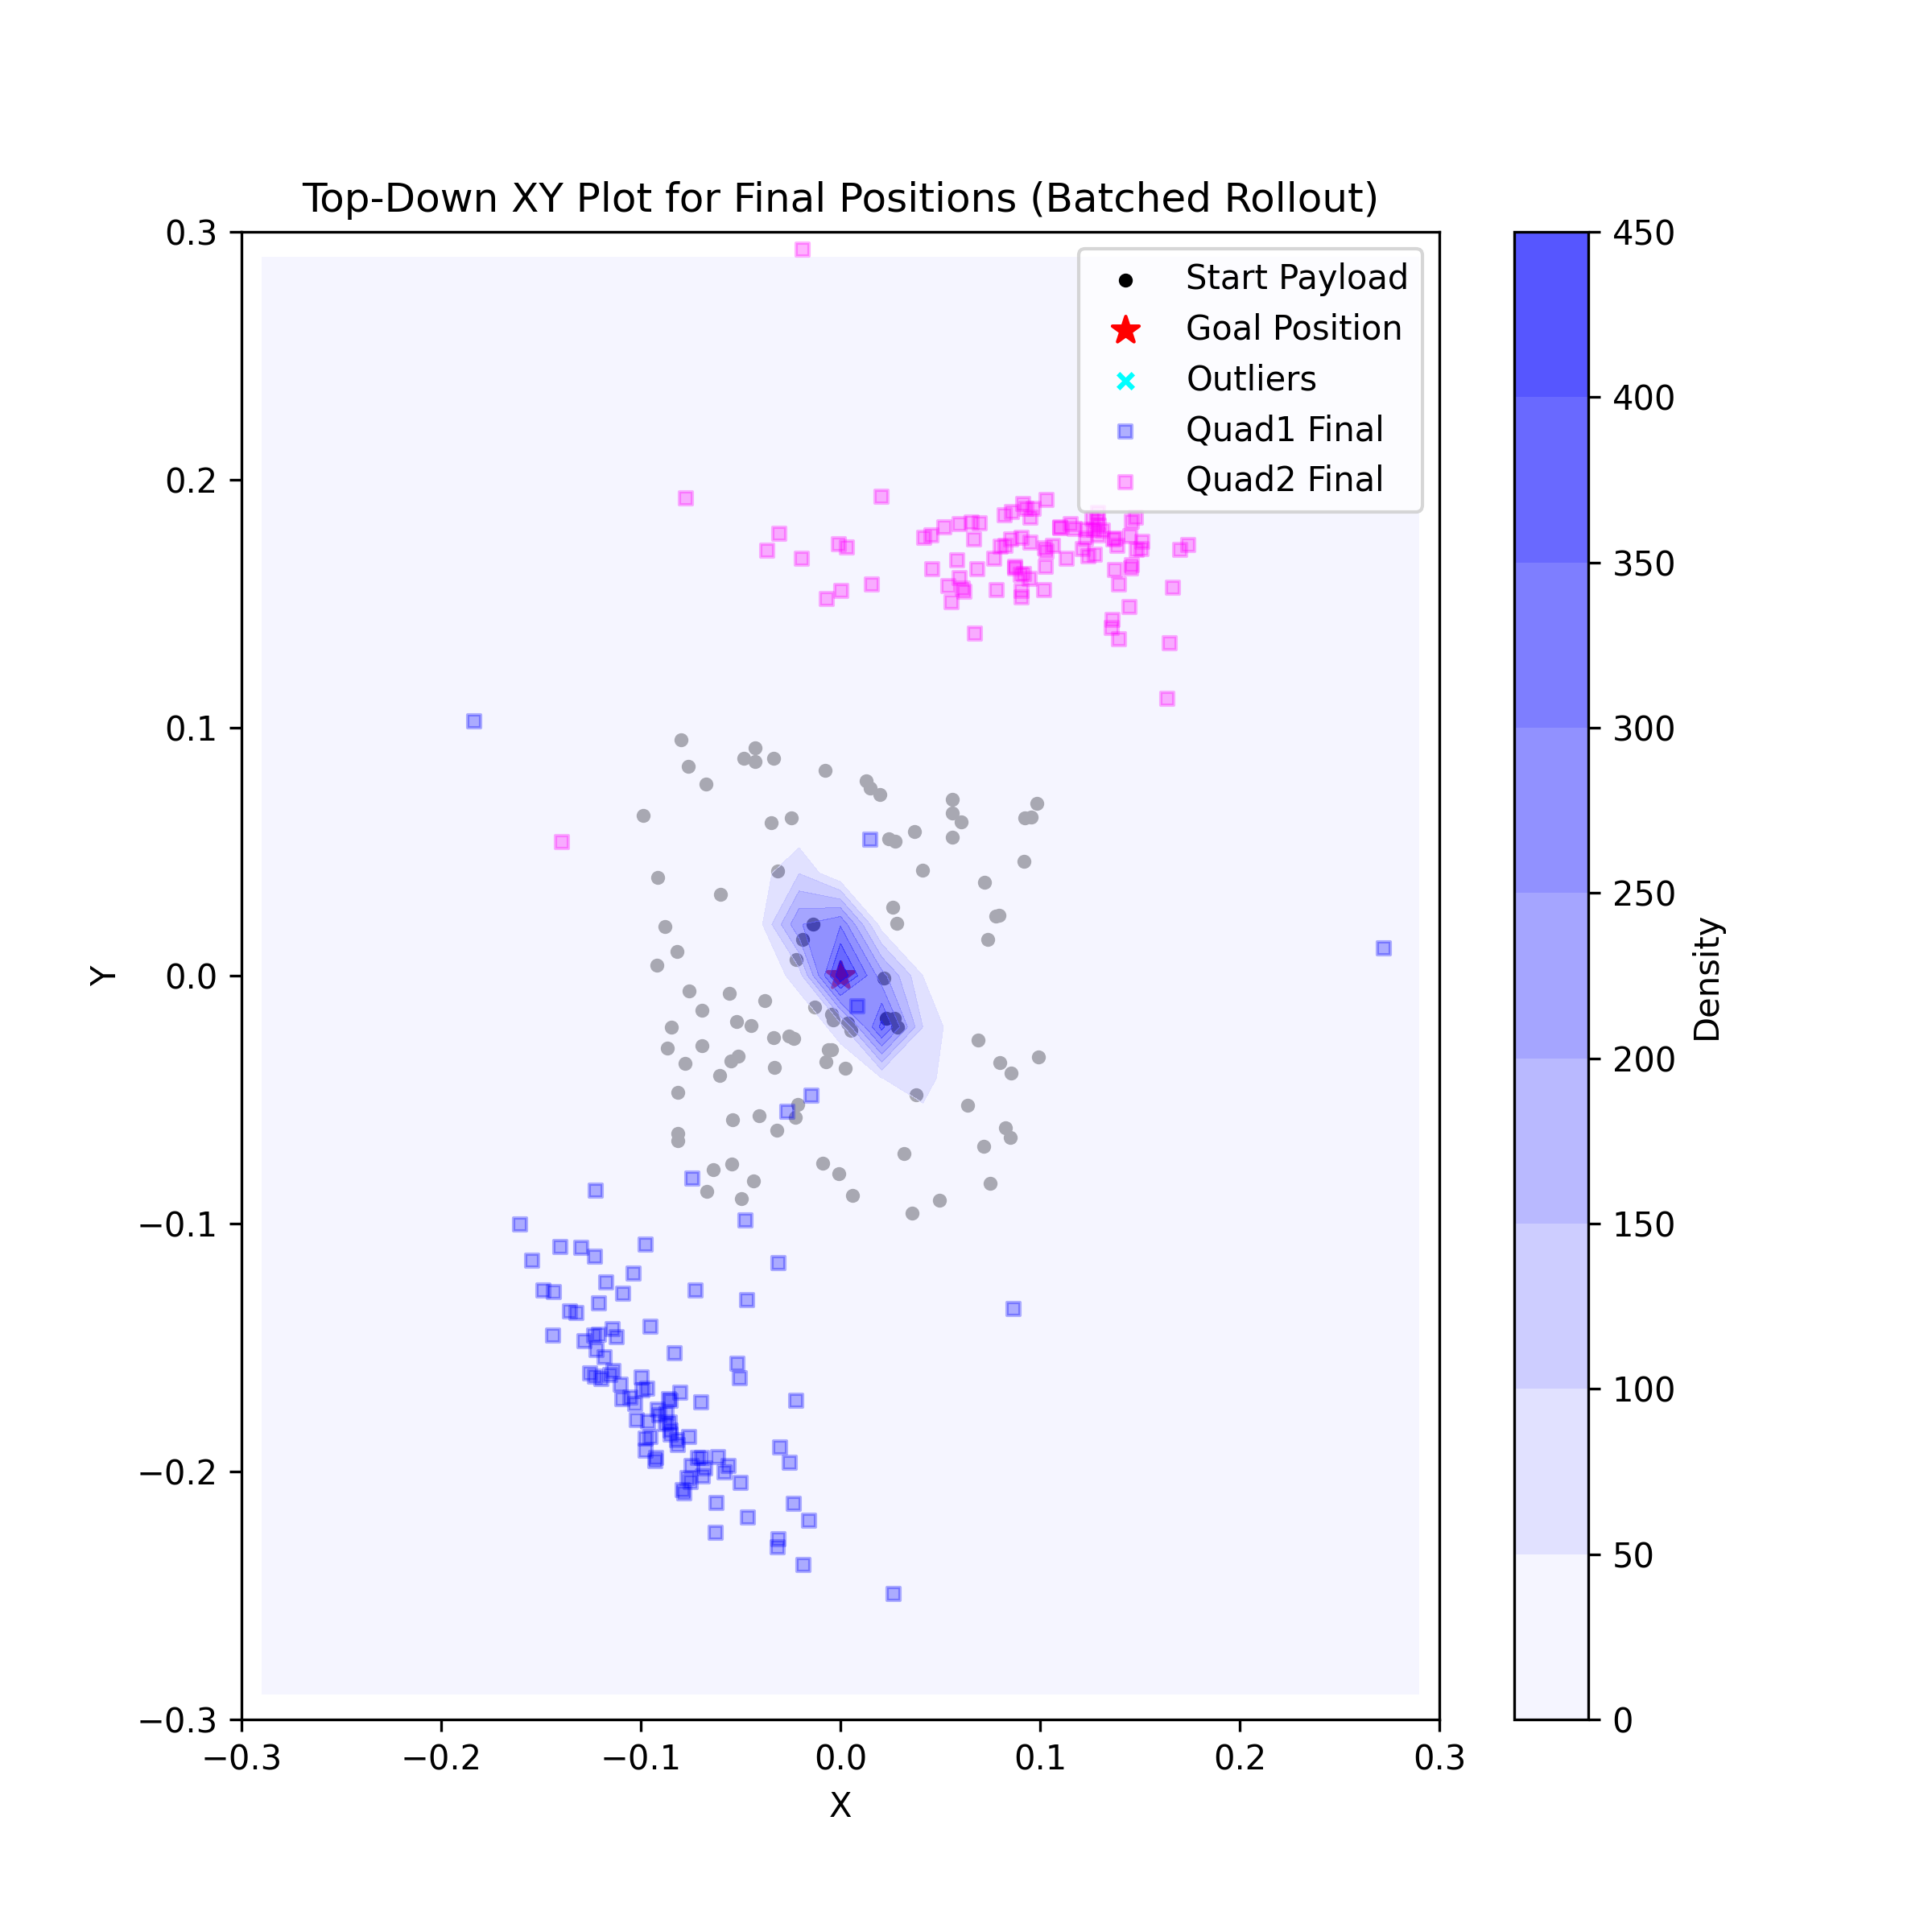
\includegraphics[width=\textwidth]{pos_recover.png}
    \caption{Single quadrotor control with payload. The quadrotor is able to recover from harsh disturbances and track a desired position.}
    \label{fig:single_quadrotor_control}
\end{figure}
\section{Multi Quadrotor Control with Payload}
\begin{itemize}
    \item Recover from harsh and track position
    \item Follow trajectory
    \item Follow trajectory with disturbance
    \item Sim2Real
\end{itemize}
\section{Policy with Limited Observations}
optional
\section{Comparison with classic control}
Compare with prev paper method \autocite{Wahba2024}